%%=============================================================================
%% Literatuurstudie
%%=============================================================================

\chapter{Literatuurstudie}
\label{ch:literatuurstudie}

\section{De IBM Z Systems omgeving}
\label{sec:De IBM Z Systems omgeving}
Het is belangrijk om te weten wat een mainframe is en wat de hoofdpunten van de technologie zijn. Het is moeilijk om een goede definitie te plakken op deze term maar het is ontwikkelt door IBM en het wordt vooral gebruikt door grote bedrijven om belangrijke applicaties te hosten en/of veel transacties te kunnen doorvoeren. Hoewel dit ook mogelijk is op een kleinschalige server, zou het resultaat niet hetzelfde zijn omdat mainframes miljarden transacties per dag zou kunnen uitvoeren zonder enige vertraging. \autocite{BasuMallick2023} \\

De mainframe wordt vaak in vergelijking gebracht met een traditionele server die je vind in een datacenter. Deze vergelijking is niet onterecht omdat ze wel een gelijkaardige functie hebben. Een mainframe zoals de hedendaagse IBM \GLS{z16} heeft de mogelijkheid om 19 miljard transacties per dag uit te voeren, wat ook verklaard waarom deze systemen gebruikt worden door 71\% van de Fortune 500 bedrijven wereldwijd. Deze machine heeft ook 40 terabyte werkgeheugen wat 1200 keer het aantal is in hedendaagse high-performance computers. \autocite{Tozzi2022} \\

De \Gls{z16} is ook `Quantum safe`: de bedreiging van Quantum computers in de toekomst blijft groeien en er is nog geen directe oplossing voor. IBM heeft hiervoor geïnvesteerd in Crypto Express 8S hardware security modules om data op de mainframe te beschermen en Quantum safe te maken. De nieuwe modules bevatten nieuwe quantum safe encryptie algoritmes die geëvalueerd zijn door de US National Institute of Standards and Technology. \autocite{Sayer2022} \\

Het is belangrijk om te weten dat de data niet wordt opgeslagen in de \GLS{ASCII} encoding maar in een binair formaat door middel van de \GLS{EBCDIC} encoding. \autocite{Singhal2023} \\ Dit is zo voor alle besturingssystemen die compatibel zijn op de mainframe behalve Linux for System z. Hierin is \GLS{ASCII} de standaard. \autocite{IBMb}


\subsection{Het hoofdbesturingssysteem z/OS}
Een IBM Mainframe ondersteund meerdere besturingssystemen maar de meest gebruikte is \GLS{z/OS}. Dit is, samen met de IBM Z Systems, ontwikkeld door IBM waardoor dit het meest compatibel is met de hardware componenten en het blijft ondersteund door IBM zelf. Deze heeft verschillende karakteristieken zoals \acrlong{wlm} (\acrshort{wlm}) om het uitvoeren van jobs in te plannen. Dit besturingssysteem kan gezien worden als hybride omdat het moderne taken van andere besturingssystemen neemt en combineerd met de architectuur van een IBM mainframe. Het heeft ook de mogelijkheid om terug te draaien naar een vorige versie zonder dat dit problemen zal veroorzaken met het systeem. \autocite{Rupp2022} 

\subsection{Software in z/OS}
Dit besturingssysteem bevat tools zoals \acrshort{tso}, \acrshort{ispf} en \acrshort{sdsf} om er een paar op te noemen. Via een 3270 terminal kan een gebruiker inloggen op de mainframe en gebruik maken van deze tools. \\

\acrlong{tso} staat voor \acrlong{tso} en is in principe de command line interface op de mainframe. Dit laat meerdere gebruikers toe om een interactieve sessie op te starten met z/OS via hun eigen inloggegevens. Zoals een traditionele CLI bestaat dit uit een prompt waar je commando's kunt ingeven om acties uit te voeren op het systeem. In \acrlong{tso} wordt dit een `READY` prompt genoemd omdat het een READY melding geeft als je commando's kunt invoeren. \autocite{IBM} \\

Hoewel TSO vrij krachtig is, zal dit door de meeste eindgebruikers gebruikt worden in combinatie met \acrshort{ispf} of \acrlong{ispf}. Dit is een GUI dat bestaat uit menu's en panelen die allemaal verschillende functies kunnen uitvoeren \autocite{IBM}. Veel gebruikte functies zijn het aanmaken en schrijven van COBOL of PL/1 programma's. \acrshort{ispf} biedt nog meer verschillende functies zoals het aanmaken van datasets tot een connectie maken met de database op de mainframe. Hierin kun je dus eigenlijk alles doen wat het platform te bieden heeft maar wel in de lijnen van de rechten die je hebt als gebruiker. \autocite{IBM} \\

\acrlong{sdsf} of \acrshort{sdsf} is volgens de \textcite{IBM2023} documentatie een interface om jobs en hun output te kunnen zien. Zo is er ook de mogelijkheid om een job te doen stoppen, bijhouden of vrijgeven. Met bijhouden wordt er bedoeld niet laten uitvoeren tot iemand een teken geef dat het uitgevoerd mag worden. Vrijgeven wordt gebruikt om de fysieke middelen zoals de CPU vrij te geven zodat een andere job deze kan gebruiken. \\ 
Het biedt ook informatie over het \gls{z/OS} systeem zodat u dit kan monitoren, managen en controleren. Hoewel het vooral gebruikt wordt om de status van een uitgevoerde job te zien, wordt deze tool ook gebruikt om fysieke toestellen te controleren (zoals een printer), de fysieke middelen zoals CPU of geheugen beheren en de system log en messages bekijken.

\subsection{Datasets}
z/OS heeft ook een andere manier om data op te slaan door middel van datasets. Dit is volgens de documentatie van \textcite{IBM} een collectie van gerelateerde data records dat opgeslagen en opgehaald wordt door een toegewezen naam. Dit zou u kunnen zien als een bestand in andere besturingssystemen zoals in Windows of Linux. \\

Hier bestaan er verschillende soorten van:

\begin{itemize}
    \item Sequentiële dataset
    \item \acrlong{pds} (\acrshort{pds})
    \item \acrlong{vsam} (\acrshort{vsam})
\end{itemize} \\

Sequentiële datasets bevatten records die achter elkaar opgeslagen zijn. Dit heeft als nadeel dat als een gebruiker bijvoorbeeld record 20 wilt lezen, moet hij eerst voorbij de voorgaande 19 records gaan. Deze soort datasets worden vooral gebruikt om grote hoeveelheden data in op te slaan. \autocite{IBM} \\

Een partitionele dataset is meer voor programma's in te schrijven. Deze dataset bevat allemaal `members` die op hun beurt dan de effectieve data bevatten. Dit heeft als voordeel dat je in een \acrshort{pds} de members kunt aanspreken in een willekeurige volgorde. Deze vorm van een dataset wordt ook wel een library genoemd. \autocite{IBM} \\

Een \acrshort{vsam} biedt een complexere manier van toegang tot verschillende soorten data en is vooral bedoeld voor applicaties. Door hun complexiteit kunnen ze niet frequent bekeken of aangepast worden zoals in \acrshort{ispf}. Een \acrshort{vsam} kun je verdelen in 4 verschillende datasets:
\begin{itemize}
    \item Key Sequence Data Set (KSDS): \\Dit komt het meest voor en zal data opslaan op basis van een key, value systeem
    \item Entry Sequence Data Set (ESDS): \\Dit houdt de records in een sequentiële volgorde bij en worden ook gelezen in deze volgorde. Dit is vooral gebruikt door databanken en z/OS Unix bestanden.
    \item Relative Record Data Set (RRDS): \\Dit houdt records bij die je kunt ophalen op basis van een nummer. Zo heb je toegang tot records die opgeslagen zijn op plaats 100 zonder dat je door de eerste 99 records moet gaan. Dit is te vergelijken met een KSDS.
    \item Lineair Data Set (LDS): \\Dit houdt data bij in een byte stream en is de enige vorm van dit soort in een traditionele z/OS file.
\end{itemize}
\autocite{IBM}
\subsection{Unix op een mainframe}
IBM heeft veel ingezet op modernisatie. Zo is er een \acrlong{uss} (\acrshort{uss}) omgeving bijgekomen die geïntegreerd is in het traditionele besturingssysteem z/OS. Er is ook een volledige mainframe die enkel Linux heeft als besturingssysteem namelijk de LinuxOne. In dit onderzoek zal er enkel gekeken worden naar een mainframe met z/OS die een \acrshort{uss} omgeving heeft. \\

Omdat de \acrshort{uss} dus samenwerkt met z/OS heb je veel meer functies die je kunt gebruiken. Zo is er de mogelijkheid op XML parsing, OpenSSH, de IBM HTTP Server for z/OS, de z/OS SDK for Java en nog veel meer. \autocite{Dhawan2013} \\
 
Dit systeem biedt een hierarchisch bestandssysteem (HFS) samen met een zSeries bestandssysteem (zFS). \autocite{Precisely2020} \\ De HFS is wel bekend voor de meeste UNIX gebruikers: Dit is een hierarchie van directories met bestanden of subdirectories die grafisch weergegeven kunnen worden in een tree view \autocite{HCLTechnologies2022}. \\ 

Zoals afgebeeld in figuur \ref{fig:HFS}, is er een root (in Unix meestal afgebeeld als '/') die directories bevat. Deze directories bevatten bestanden en andere directories. Ze kunnen ook andere informatie bevatten over deze bestanden. Directories die opgeslagen zijn in een andere directorie worden subdirectories genoemd. Vaak wordt er ook gebruik gemaakt van een parent-child verwijzing waar de parent directorie een level boven de child of subdirectorie zit. \autocite{Codecadamy2022} \\

\begin{figure}[pt!]
    \centering
    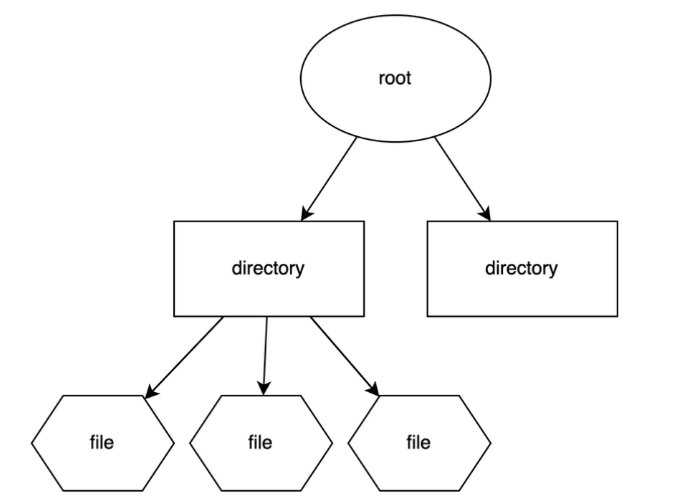
\includegraphics[width=300pt]{./graphics/HFS.png}
    \caption{HFS voorbeeld \autocite{Codecadamy2022}}
    \label{fig:HFS}
\end{figure}

zFS is iets minder bekend en kan gebruikt worden in plaats van of als toevoeging op het traditionele HFS. Dit heeft vooral zijn waarde door zijn sterke performantie in bestanden die vaak worden gebruikt. Het verminderd ook het risico van het verlies in updates omdat het data asynchroon schrijft in plaats van te wachten op een sync interval. Bestanden in dit systeem kunnen aangepast worden door middel van een Application Programming Interface (API) en kunnen zelf in de HFS toegevoegd worden zonder enige problemen. \autocite{IBM2012} \\

\begin{figure}[pt!]
    \centering
    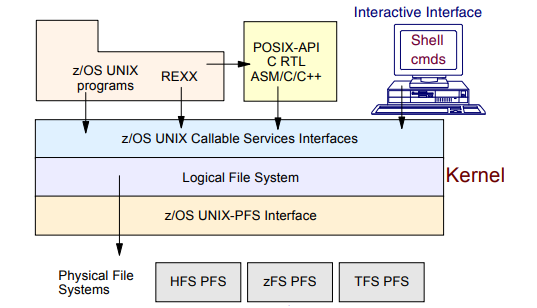
\includegraphics[width=300pt]{./graphics/zFS.png}
    \caption{zFS werking \autocite{IBM2012}}
    \label{fig:zFS}
\end{figure}

In figuur \ref{fig:zFS} worden de bestanden opgehaald vanuit het zFS bestandsysteem door middel van de interactieve interface. Doankzij de API's tussen het logische -en fysieke bestandsysteem worden de juiste bestanden opgehaald en teruggegeven aan de gebruiker. \\

Unix bestanden op de mainframe worden bijna op dezelfde manier gebruikt als op een traditioneel unix systeem. Het kan een Java, C++ of Python programma bevatten. Deze programma's kunnen ook bestanden lezen of schrijven in een JSON of YAML formaat. Die kunnen op hun beurt dan gebruikt worden om analyses te doen op bepaalde data. Het hangt dus allemaal af van de use case om te zien op welke manier deze unix bestanden het best gebruikt worden. \autocite{Precisely2020}

\subsection{Python AI toolkit for z/OS}
Omdat we een Python interpreter zullen opzetten, zal er hier vooral gefocust worden op Python in z/OS. In Python wordt er vaak gebruik gemaakt van externe packages die publiek beschikbaar zijn. Deze moeten wel geïnstalleerd zijn op het systeem om er gebruik van te maken en dit kan een probleem zijn in \acrshort{uss}. Door de beveiliging in een mainframe is het niet altijd even makkelijk om packages of andere direct te installeren in z/OS \autocite{IBM2021} en hierdoor heeft IBM een Python AI toolkit for z/OS opgezet. \\

In de aankondiging door Evan \textcite{Rivera2023} werd deze toolkit beschreven als een bekende en flexibele ervaring voor developers tijdens het ontwerpen van AI oplossingen. Het biedt open source software en deze kunnen eenvoudig geïnstalleerd worden door de Package Installer for Python (pip). \\

De Python AI toolkit is dus een bibliotheek met verschillende, wereldwijd gebruikte Python packages voor AI en Machine learning workloads bijvoorbeeld NumPy, SciPy, Jupyter, etc. Elk van deze packages is volledig onderzocht geweest voor potentiële problemen in het systeem waardoor alles in deze toolkit voldoet aan de beveiligingsvoorwaarden zoals andere z/OS producten. \autocite{Bostian2023}

\subsection{Andere besturingssystemen}
Zoals eerder vermeld is z/OS niet het enige besturingssysteem dat beschikbaar is op de mainframe. Hoewel dit door IBM aangeboden wordt, zijn er andere mogelijkheden die elk hun eigen sterktes en zwaktes hebben. \\

\begin{itemize}
    \item z/Virtual Machine (z/VM)\\
    Dit is een type 1 hypervisor en kan gebruikt worden om meerdere besturingssystemen in te hosten. Dit bestaat uit een control program (cp) en een conversation monitoring system (CMS). De cp is verantwoordelijk voor het creëren van meerdere virtuele machines op basis van de fysieke hardware middelen. Het zorgt ook voor data en applicatie beveiliging voor alle systemen die in het systeem zitten. De CMS zit in een eigen virtuele machine en biedt een interactieve sessie tussen de andere virtuele machines en eindgebruikers. \autocite{IBMb} \\
    
    \item z/Virual Storage Extended (z/VSE) \\
    Dit besturingssysteem is vooral nuttig voor kleinere bedrijven die geen complexe batch -of transactie jobs moeten processen. Het is mogelijk dat naarmate ze groeien, ze overgaan naar z/OS als z/VSE niet genoeg blijkt te zijn. Het design van dit besturingssysteem maakt het perfect voor meer routine batch jobs parallel uit te voeren. Meestal wordt z/VM ook gebruikt als een terminal interface voor development en systeembeheer in z/VSE. \autocite{IBMb} \\
    
    \item Linux for System z \\
    Dit is zoals de naam zegt, Linux op de mainframe. Er zijn hier 2 verschillende distributies voor: Linux for S/390 (gebruikt 31-bit adressering) en Linux for System z (gebruikt 64-bit adressering) \\
    Linux for System Z refereerd naar Linux for S/390. Dit besturingssysteem maakt niet gebruik van een 3270 terminal maar X-Windows based terminals. Dit bestaat uit een cli waarmee je meestal een telnet of ssh connectie maakt met het Linux for System z besturingssysteem. Dit is ook volledig in de encoding ASCII en niet EBCDIC. \autocite{IBMb} \\
    
    \item z/Transaction Processing Facility (z/TPF) \\
    Dit besturingssysteem is vooral nuttig voor bedrijven die veel transacties moeten uitvoeren zoals een bank of vliegmaatschappij. Dit kan gebruik maken van verschillende mainframes om tienduizende transacties per seconde uit te voeren zonder enige onderbreking. \autocite{IBMb}
\end{itemize}


\section{IBM Developer for z/OS}
\label{sec:IBM Developer for z/OS (IDz)}
\subsection{IDz}
De testomgeving waarin we zullen werken is IBM Developer for z/OS (IDz) versie 16.0.2. Dit programma is volgens de definitie van \textcite{Spohn2023} een toolset voor het ontwikkelen en opzetten van hybride cloud applicaties op z/OS. \\
Het is een Eclipse based programma met de mogelijkheid om een connectie te maken met verschillende omgevingen op de mainframe (bv de \acrshort{uss} of z/OS omgeving). Zo kunt u alle bestanden zien, openen en aanpassen. Omdat de data nogsteeds op de mainframe staat, kunnen wijzigingen direct gezien worden ookal bekijkt u het in een ander programma. Als u bijvoorbeeld een bestand wijzigt via IDz, kunt u de wijzigingen direct zien in \acrshort{ispf}. \\
Dit programma is vooral ontwikkelt om een envoudige IDE te bieden om in te programmeren aangezien niet iedereen bekend is met \acrshort{ispf}. \\

Zoals vermeld zal er gebruik worden gemaakt van IDz versie 16.0.2 . In het overzicht van \textcite{IBM2024}, ondersteund deze versie syntax veranderingen voor COBOL 6.4, PL/1 6.1 en REXX. Er is ook een ZUnit update wat vooral het gebruik van deze tool makkelijker maakt. \\

ZUnit staat voor z/OS Automated Unit Testing en is een framework dat gebruikt wordt in IDz om COBOL en PL/1 programma's te testen. Hiervoor maakt het gebruik van verschillende `samples` die door IBM ontworpen zijn (bv. Enterprise COBOL CALL02.cbl sample test case). Het gebruik van deze tool maakt het makkelijker voor developers om hun code (geschreven in COBOL of Pl/1) te testen op de mainframe. Dit maakt het schrijven van code in IDz veel efficiënter. \autocite{IBM2024a}

\subsection{Eclipse IDE}
zoals eerder vermeld is IDz gebaseerd op de Eclipse Integrated Development Environment (IDE) wat ontwikkeld is door de Eclipse Foundation in 2001. Het is begonnen sinds IBM 3 miljoen lijnen code van hun Java tools heeft gedoneerd om een open source IDE te creëren. Het is dus Java gebaseerd maar is kan nogsteeds gebruikt worden voor andere programeertalen zoals Python door de verschillende plug-ins die beschikbaar zijn gemaakt door de community achter Eclipse. \autocite{Hanna2021} \\

Eclipse zelf heeft ook de mogelijkheid om verder uit te breiden door plug-ins. Dit zijn toevoegingen aan de gebruikte software die het mogelijk maken om applicaties, computer programma's en web browsers aan te passen. Dit zijn ook add ons die extra functionaliteiten kunnen bieden aan het gebruikte programma. \autocite{George2021}

\subsection{Wizards}
Een programma zoals IDz heeft veel mogelijkheden om instellingen aan te passen door middel van wizards. Dit is een serie van pagina's dat de gebruiker begeleidt om een complexe taak uit te voeren. Elke pagina vraagt wat informatie en als de gebruiker op 'finish' klikt wordt de taak uitgevoerd. Er is ook altijd een mogelijkheid om het proces stop te zetten. \autocite{Eclipse2006}

\section{IBM Z in een bankomgeving}
Dit onderzoek wordt uitgevoerd in een bankomgeving dus is het wel interessant om na te gaan welke voordelen deze technologie te bieden heeft in deze omgeving. \\ 

Volgens \textcite{Turner2022} gebruiken de meeste banken een IBM mainframe omdat ze de rekenkracht kunnen bieden die banken nodig hebben om efficiënt te kunnen werken. Kenmerken zoals robuustheid, betrouwbaarheid en snelle processing kracht spelen ook een grote rol aangezien het van groot belang is dat het systeem bijna altijd actief moeten zijn. De mainframe toont hier zijn sterkte door de 8 nines oftwel 99,999999\% van de tijd beschikbaar per jaar. \autocite{IBMa} \\

Dit is niet de enige reden waarom het gebruikt wordt door 92 van de top 100 banken ter wereld \autocite{Tozzi2022}. In een aankondiging van \textcite{IBM2022} over hun nieuw systeem de IBM z16, werd er gezegd dat 70\% van wereldwijde transacties door een mainframe verwerkt worden. \\

Beveiliging speelt ook een grote rol, een studie van \textcite{MorningConsult2022} toont aan dat krediet kaart fraude het meest voorkomende type fraude is onder klanten in 7 verschillende landen waaronder Duitsland, de Verenigde Staten en China. de IBM zSystems heeft al een goede transactie beveiliging zonder teveel vertraging maar de z16 brengt hier nog een AI model bij. Hierdoor kunnen banken transacties controleren op een veel grotere schaal: 300 miljard door AI beveiligde transacties per dag met maar 1 milliseconde vertraging. Andere zaken zoals belastingsfraude kunnen ook vermeden worden hiermee. \autocite{IBM2022} \\

IBM doet dit door middel van een nieuwe Telum Processor. Het is ontworpen om deep learning algoritmes naar workloads te brengen voor bedrijven om in real-time fraude te detecteren en te verwerpen. Dit is de eerste processor van IBM dat gebruik maakt van AI terwijl de transactie wordt uitgevoerd. Naast het detecteren van fraude is deze chip nog nuttig voor loan processing, het tegengaan van witwassen van geld en risico analyse. \autocite{IBM2021a} \\

Batch processen is ook een belangrijk voordeel dat een mainframe te bieden heeft. Dit zijn jobs die uitgevoerd kunnen worden met weinig of geen interactie van een gebruiker \autocite{IBM}. Dit is vooral nuttig voor taken die op vaste momenten moeten uitgevoerd worden. In figuur \ref{fig:batch} is een duidelijk voorbeel over hoe een batch job te werk gaat:

\begin{itemize}
    \item[1] De batch job wordt opgestart door de mainframe
    \item[2] De job genereert statistieken van het bedrijf
    \item[3] Er wordt een backup gemaakt van de kritische bestanden en de database voor en na de job
    \item[4] De statistieken worden verstuurd naar een specifieke plaats zodat het geanalyseerd kan worden
    \item[5] Fouten in de statistieken worden in een andere locatie geplaatst
    \item[6] Informatie van klanten hun bankrekening wordt gemaakt en verstuurd.
    \item[7] Een verslag van de processing tijd wordt verstuurd naar de partners van de bank
    \item[8] De partner ontvangt het verslag
    \item[9] Het systeem monitort de uitkomst van de batch job
    \item[10] Jobs en transacties updaten de database zodat de progressie wordt opgeslagen
\end{itemize}
\\ \\
\begin{figure}[p!]
    \centering
    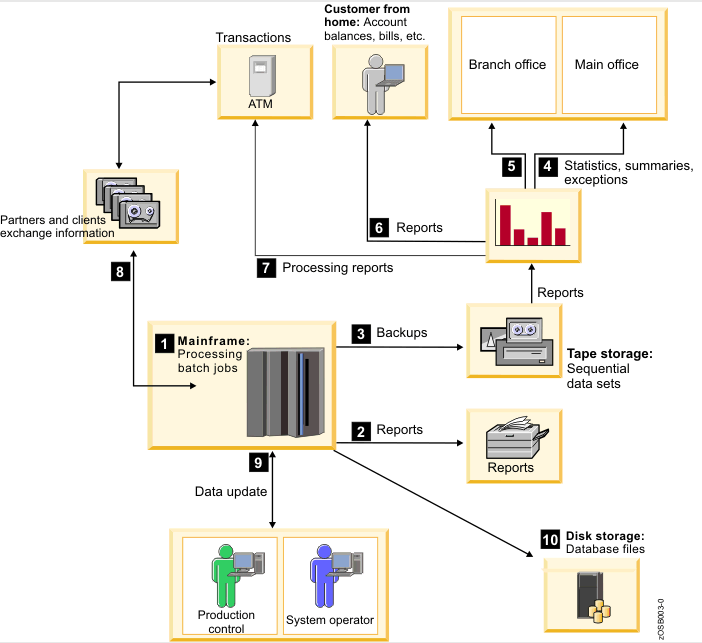
\includegraphics[width=400pt]{./graphics/BatchJobVB.png}
    \caption{Batch Job \autocite{IBMb}}
    \label{fig:batch}
\end{figure}

\begin{figure}[ph!]
    \centering
    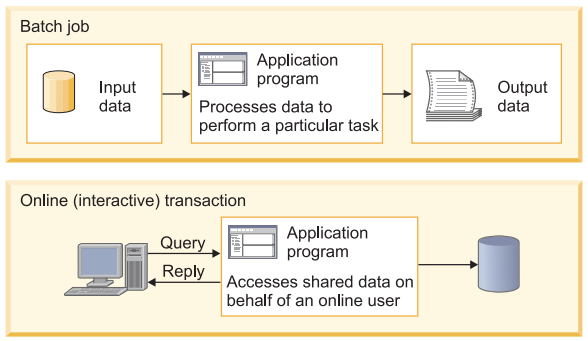
\includegraphics[width=400pt]{./graphics/BatchVSOnline.png}
    \caption{Grafisch verschil tussen batch en OLTP \autocite{IBMb}}
    \label{fig:online}
\end{figure}

Batch jobs zijn niet de enige vorm van jobs die uitgevoerd worden op een mainframe. Online transaction processing of OLTP is zeer belangrijk in een bank. In contrast met batch processing, heeft dit een eindgebruiker nodig die de job opstart. Het heeft ook geen vast moment waarop de job uitgevoerd wordt en kan dus op elk moment van de dag. Meestal duren deze transacties niet lang maar de systemen die verantwoordelijk zijn om deze jobs uit te voeren moeten veel verschillende gebruikers op hetzelfde moment ondersteunen zonder enige vertraging. \autocite{IBMb} \\

Een grafische voorstelling van de verschillen tussen een batch job en een online transaction job vind u in figuur \ref{fig:online}. Een batch job heeft dus input die verwerkt wordt door een programma op een bepaald, vast moment. De uitkomst wordt dan geschreven in een bestand om analyses op uit te voeren. \\
Een online transactie daarentegen wacht op een query van een gebruiker om te starten. Data wordt dan opgehaald uit het systeem en teruggegeven aan de gebruiker. \autocite{IBMb}


